
\section{\trCompact{}性的证明}
\label{sec:compactness-proof}

现在我们来证明定理 6.5.4。正如我们已经注意到的（注记 6.4.1），当 $H$ 为零时，\trFloerEquation{}不是别的，正是一个\trCauchyRiemann{}方程，它的解恰好就是由\trGromov~[42] 引入的那些 $J$-\trHolomorphic{}曲线。\trGromov{}的\trCompact{}性定理（另见 [62]）在我们这个\trHamiltonian{}非零的情形下依然成立。就本节而言，我们相当贴近地依循 [49] 的讲述。

\begin{remark}\label{thm:asphericity-important-compactness}
我们已经用\trAsphericity{}\cref{thm:symplectic-asphericity}来定义\trActionFunctional。我们将会看到，它对于\trCompact{}性而言是一个重要的条件（我们将确切解释在何处用到它）。
\end{remark}

该定理是下面这个命题的一个推论。

\begin{proposition}\label{thm:uniform-gradient-bound}
在\cref{thm:symplectic-asphericity}（即 $\langle[\omega],\pi_2(W)\rangle=0$）之下，存在一个常数 $A>0$ 使得
\[
\forall u\in\scr{M},\ \forall(s,t)\in\RR\times S^1,\qquad
\bigl\|\operatorname{grad}_{(s,t)}u\bigr\|\le A\text{。}
\]
\end{proposition}

\begin{proof}[定理 6.5.4 的证明]
与前面一样，我们的策略是证明：给定 $\scr{M}$ 的一个序列 $u_n$，就有下列结果：
\begin{itemize}
\item 首先，$u_n$ 容许一个在 $\cC^0_{\mathrm{loc}}(\RR\times S^1;W)$ 中\trConvergence{}到 $u_0$ 的子序列。
\item 其次，极限 $u_0$ 是 $\cC^\infty$ 类的，并且是\trFloerEquation{}的一个解。
\item 最后，$u_n$ 在 $\cC^\infty(\RR\times S^1;W)$ 中确实趋于 $u_0$。
\end{itemize}
\cref{thm:uniform-gradient-bound}给出了 $\scr{M}$ 中元素的\trEquicontinuity{}性。于是，$\scr{M}$ 在从 $\RR\times S^1$ 到 $W$ 的连续映射组成的集合中的闭包是\trCompact{}的（仍然是借助\trArzelaAscoliTheorem），这就完成了第一步。一个\trEllipticRegularity{}论证使我们得以证明后两步。注意，我们不能使用命题 6.5.3，因为 $u_0$ 只是连续的；我们将需要一个更一般的陈述，它会在引理 12.1.1 中给出。最后，由命题 12.1.4，$\cC^0_{\mathrm{loc}}$ 与 $\cC^\infty_{\mathrm{loc}}$ 这两个\trTopology{}在 $\scr{M}$ 上相重合。因此，这个\trManifold{}对于 $\cC^\infty$ \trTopology{}也是\trCompact{}的。
\end{proof}

\begin{proof}[\cref{thm:uniform-gradient-bound}的证明]
设 $u\colon\RR\times S^1\to W$ 是一个解。把它看成从 $\RR\times\RR$ 到 $W$ 的一个（关于变量 $t$ 为\trPeriodic{}的）映射要更方便些，我们也就这么做。我们给出一个反证法证明，即假设命题的结论不真。这意味着，存在 $\scr{M}$ 中元素的一个序列 $(u_k)$ 与 $\RR^2$ 中元素的一个序列 $(s_k,t_k)$，使得
\[
\lim_{k\to\infty}\bigl\|\operatorname{grad}_{(s_k,t_k)}u_k\bigr\|=+\infty\text{。}
\]
因此在这个证明中，我们考虑 $\scr{M}$ 的一个发散的序列，并且来证明：它事实上将产生某个在我们的假设下禁止其存在的东西，也就是\cref{fig:bubble-rescaling}与\cref{fig:bubble-neck}所展示的那个\trBubble。

设 $(\varepsilon_k)$ 是一列趋于 $0$ 的正数，使得
\[
\lim_k\varepsilon_k\bigl\|\operatorname{grad}_{(s_k,t_k)}u_k\bigr\|=+\infty\text{。}
\]
我们对函数 $g=\|\operatorname{grad}u\|$ 应用下面这个名叫“半极大值”引理的引理\footnote{这是这个理论中的一个经典引理。它的起源似乎出自 Ekeland；他的书 [26] 第 IV 章的开头就包含有这一主题的种种变奏。}。

\begin{lemma}\label{thm:half-maximum-lemma}
设 $g\colon X\to\RR^+$ 是完备\trMetric{}空间上的一个连续函数。设 $x_0\in X$ 且 $\varepsilon_0>0$。则存在 $y\in X$ 与 $\varepsilon\in\left]0,\varepsilon_0\right]$，使得
\[
\left\{\begin{array}{l}
d(y,x_0)\le 2\varepsilon\\
\varepsilon g(y)\ge \varepsilon_0 g(x_0)\\
g(x)\le 2g(y)\qquad\ \ \forall x\in B(y,\varepsilon)\text{。}
\end{array}\right.
\]
\footnote{译注：原书首行印作 $d(y,x_0)\le 2\varepsilon$；但据证明中的迭代（$x_n\in B(x_{n-1},\varepsilon_{n-1})$，$\varepsilon_n=\varepsilon_{n-1}/2$），至多只能得到 $d(y,x_0)<\varepsilon_0+\varepsilon_1+\cdots+\varepsilon_{N-1}<2\varepsilon_0$（几何级数），除首例 $y=x_0$、$\varepsilon=\varepsilon_0$ 外一般达不到 $2\varepsilon$。数例：取 $X=\RR$、$x_0=0$、$\varepsilon_0=1$、$g(x)=e^{4x}$，按证明的迭代得 $x_1=0.3$、$x_2=0.6$，至 $y=x_3=0.8$ 与 $\varepsilon=\varepsilon_3=1/8$ 方才适定；此时 $d(y,x_0)=0.8>2\varepsilon=0.25$，却有 $d(y,x_0)\le 2\varepsilon_0=2$。故首行疑应作 $d(y,x_0)\le 2\varepsilon_0$。此处照原书排印，存疑备案（下面的重标度论证只用到后两行，不受影响）。——译者注}
\end{lemma}

\begin{proof}
若在整个球 $B(x_0,\varepsilon_0)$ 上都有 $g(x)\le 2g(x_0)$，那就什么也不必做，只需取 $y=x_0$ 与 $\varepsilon=\varepsilon_0$。若情形并非如此，则在该球中存在一点 $x_1$ 使得 $g(x_1)>2g(x_0)$。令 $\varepsilon_1=\varepsilon_0/2$。于是就有
\[
\varepsilon_1g(x_1)>\varepsilon_0g(x_0)\text{。}
\]
若 $x_1$ 与 $\varepsilon_1$ 合适，那我们就大功告成了。否则，我们继续下去。照此办理，我们构造出该球中点的一个序列 $x_n$ 与正数的一个序列 $\varepsilon_n$，使得
\[
\left\{\begin{array}{l}
\varepsilon_n=\dfrac{\varepsilon_{n-1}}{2}\\[2pt]
\varepsilon_n g(x_n)\ge \varepsilon_0 g(x_0)\text{。}
\end{array}\right.
\]
显然，第一行使 $\varepsilon_n$ 趋于 $0$，而 $x_n$ 趋于一个极限（我们的空间是完备的），于是第二行禁止这一过程无休止地继续下去：经过有限多次尝试之后，我们终将找到合适的 $x_n$ 与 $\varepsilon_n$。
\end{proof}

这个引理给出了一列（另一列）$\varepsilon_k$ 与一列（另一列）$(s_k,t_k)$，使得
\[
\lim_{k\to\infty}\varepsilon_k\bigl\|\operatorname{grad}_{(s_k,t_k)}u_k\bigr\|=+\infty
\]
并且
\[
2\bigl\|\operatorname{grad}_{(s_k,t_k)}u_k\bigr\|\ge
\bigl\|\operatorname{grad}_{(s,t)}u_k\bigr\|\qquad
\text{对 }(s,t)\in B\bigl((s_k,t_k),\varepsilon_k\bigr)\text{。}
\]
令 $R_k=\bigl\|\operatorname{grad}_{(s_k,t_k)}u_k\bigr\|$；则 $\varepsilon_kR_k\to+\infty$，并且
\[
v_k(s,t)=u_k\Bigl(\frac{(s,t)}{R_k}+(s_k,t_k)\Bigr)\text{，}
\]
于是
\[
\operatorname{grad}_{(s,t)}v_k=\frac{1}{R_k}\operatorname{grad}_{\frac{(s,t)}{R_k}+(s_k,t_k)}u_k\text{，}
\]
特别地，对于 $(s,t)=(0,0)$，我们有
\[
\operatorname{grad}_{(0,0)}v_k=\frac{1}{R_k}\operatorname{grad}_{(s_k,t_k)}u_k\text{。}
\]
这样一来，由构造有 $\bigl\|\operatorname{grad}_{(0,0)}v_k\bigr\|=1$，并且在 $B(0,\varepsilon_kR_k)$ 上，
\[
\bigl\|\operatorname{grad}_{(s,t)}v_k\bigr\|
=\frac{1}{R_k}\Bigl\|\operatorname{grad}_{\frac{(s,t)}{R_k}+(s_k,t_k)}u_k\Bigr\|
\le\frac{2}{R_k}\bigl\|\operatorname{grad}_{(s_k,t_k)}u_k\bigr\|\le 2\text{，}
\]
故\trGradient{}是\trUniform{}\trBounded{}的。最后，$u_k$ 都是解，因此 $v_k$ 满足
\[
\frac{\partial v_k}{\partial s}+J(v_k)\frac{\partial v_k}{\partial t}
+\frac{1}{R_k}\operatorname{grad}_{\left(t_k+\frac{t}{R_k},\ v_k\right)}H=0\text{。}
\]
现在我们应用\trEllipticRegularity{}引理（引理 12.1.1）；在必要时抽取一个子序列之后，序列 $v_k$ 趋于一个极限 $v$，它属于 $\cC^\infty_{\mathrm{loc}}(\RR^2;W)$，并且是\trFloerEquation{}的一个解。此外，
\[
\left\{\begin{array}{ll}
\bigl\|\operatorname{grad}_{(0,0)}v\bigr\|=1\text{，} & \text{特别地，$v$ 不是常值的，}\\[2pt]
\bigl\|\operatorname{grad}_{(s,t)}v\bigr\|\le 2 & \text{对一切 }(s,t)\in\RR^2\text{，}\\[2pt]
\dfrac{\partial v}{\partial s}+J(v)\dfrac{\partial v}{\partial t}=0\text{，} & \text{从而 $v$ 是 $J$-\trHolomorphic{}的。}
\end{array}\right.
\]

最后我们来证明 $v$ 的\trEnergy{}是有限的。设 $B_k=B\bigl((s_k,t_k),\varepsilon_k\bigr)$。我们有
\[
\begin{aligned}
\int_{B(0,\varepsilon_kR_k)}\bigl\|\operatorname{grad}v_k\bigr\|^2
&=\int_{B_k}\bigl\|\operatorname{grad}u_k\bigr\|^2\,dt\,ds\\
&=\int_{B_k}\Bigl(\Bigl\|\frac{\partial u_k}{\partial s}\Bigr\|^2+\Bigl\|\frac{\partial u_k}{\partial t}\Bigr\|^2\Bigr)dt\,ds\\
&=\int_{B_k}\Bigl(\Bigl\|\frac{\partial u_k}{\partial s}\Bigr\|^2+\Bigl\|\frac{\partial u_k}{\partial t}-X_t(u_k)+X_t(u_k)\Bigr\|^2\Bigr)dt\,ds\\
&\le\int_{B_k}\Bigl(\Bigl\|\frac{\partial u_k}{\partial s}\Bigr\|^2+\Bigl\|\frac{\partial u_k}{\partial t}-X_t(u_k)\Bigr\|^2\Bigr)dt\,ds\\
&\qquad+\int_{B_k}\Bigl(\bigl\|X_t(u_k)\bigr\|^2+2\Bigl\|\frac{\partial u_k}{\partial t}-X_t(u_k)\Bigr\|\,\bigl\|X_t(u_k)\bigr\|\Bigr)dt\,ds\\
&\le\int_{B_k}\Bigl(\Bigl\|\frac{\partial u_k}{\partial s}\Bigr\|^2+2\Bigl\|\frac{\partial u_k}{\partial t}-X_t(u_k)\Bigr\|^2+2\bigl\|X_t\bigr\|^2\Bigr)dt\,ds\\
&\le 3E(u_k)+2\int_{B_k}\bigl\|X_t\bigr\|^2\,dt\,ds\le 3C+2\int_{B_k}\bigl\|X_t\bigr\|^2\,dt\,ds\text{，}
\end{aligned}
\]
其中 $C$ 是由推论 6.5.9（它是命题 6.5.7 的一个推论）给出的常数。

当 $k$ 趋于无穷时，最后一个积分趋于 $0$（$B_k$ 是半径 $\varepsilon_k$ 趋于 $0$ 的一个球），于是对充分大的 $k$，
\[
\int_{B(0,\varepsilon_kR_k)}\Bigl(\Bigl\|\frac{\partial v_k}{\partial s}\Bigr\|^2+\Bigl\|\frac{\partial v_k}{\partial t}\Bigr\|^2\Bigr)\le 4C
\]
而在极限中，$B(0,\varepsilon_kR_k)$ \trCovering{}了整个 $\RR^2$，于是由 Fatou 引理\footnote{例如参见 [64]。}，$v$ 的\trEnergy{}是有限的。

我们正亲眼目睹一个“\trBubble”的形成，而它将被我们关于\trSphere{}的假设所禁止：在点 $(s_k,t_k)$ 附近，半径为 $\varepsilon_k$ 的球的边界回路越来越小，而 $u_k$ 在这一点的\trGradient{}却在爆炸。这正是我们为何选取了一个新的\trParametrization{}（即使用 $\varepsilon_kR_k$ 的小技巧）的缘由，如\cref{fig:bubble-rescaling}所示。

\begin{figure}[htbp]
\centering
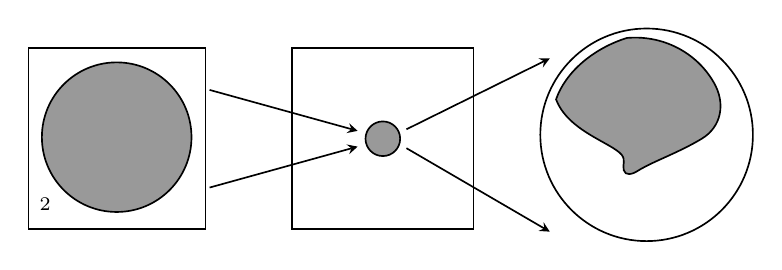
\begin{tikzpicture}[>=stealth,line width=0.6pt]
  \draw (-4.5,-1.15) rectangle (-2.25,1.15);
  \filldraw[fill=black!40] (-3.38,0.02) circle (0.95);
  \node at (-4.28,-0.9) {$\RR^2$};
  \draw (-1.15,-1.15) rectangle (1.15,1.15);
  \filldraw[fill=black!40] (0,0) circle (0.22);
  \draw (3.35,0.05) circle (1.35);
  \filldraw[fill=black!40]
    (2.2,0.5) .. controls (2.32,0.85) and (2.68,1.15) .. (3.1,1.28)
    .. controls (3.55,1.32) and (3.98,1.1) .. (4.2,0.72)
    .. controls (4.36,0.45) and (4.3,0.15) .. (4.05,0.0)
    .. controls (3.75,-0.18) and (3.45,-0.28) .. (3.25,-0.4)
    .. controls (3.16,-0.46) and (3.08,-0.47) .. (3.06,-0.4)
    .. controls (3.04,-0.33) and (3.09,-0.27) .. (3.03,-0.2)
    .. controls (2.9,-0.05) and (2.35,0.1) .. (2.2,0.5) -- cycle;
  \draw[->] (-2.2,0.62) -- (-0.32,0.1);
  \draw[->] (-2.2,-0.62) -- (-0.32,-0.1);
  \draw[->] (0.3,0.12) -- (2.12,1.02);
  \draw[->] (0.3,-0.12) -- (2.12,-1.18);
\end{tikzpicture}
\caption{}
\label{fig:bubble-rescaling}
\end{figure}

既然一个清楚的计算胜过一长篇大论，我们现在就来估计 $v$ 的像的辛面积。

\begin{lemma}\label{thm:symplectic-area-nonzero}
$v$ 的辛面积有限且非零。
\end{lemma}

\begin{proof}
\[
\begin{aligned}
\int_{\RR^2}v^\star\omega
&=\int_{\RR^2}\omega\Bigl(\frac{\partial v}{\partial s},\ \frac{\partial v}{\partial t}\Bigr)ds\,dt\\
&=\int_{\RR^2}\omega\Bigl(-J(v)\frac{\partial v}{\partial t},\ \frac{\partial v}{\partial t}\Bigr)ds\,dt
\qquad\text{因为 }\frac{\partial v}{\partial s}=-J(v)\frac{\partial v}{\partial t}\text{，}\\
&=\int_{\RR^2}\omega\Bigl(\frac{\partial v}{\partial t},\ J(v)\frac{\partial v}{\partial t}\Bigr)ds\,dt\\
&=\int_{\RR^2}\Bigl\|\frac{\partial v}{\partial t}\Bigr\|^2ds\,dt<+\infty
\end{aligned}
\]
这里用到了上面的估计\footnote{译注：原书 because 从句印作“$\frac{\partial v}{\partial t}=-J(v)\frac{\partial v}{\partial s}$”，与本证明上一行所据的 $J$-\trHolomorphic{}方程 $\frac{\partial v}{\partial s}+J(v)\frac{\partial v}{\partial t}=0$ 不符（两个导数倒置）；此处径改。——译者注}。此外，这一面积非零，因为 $v$ 不是常值的。
\end{proof}

\begin{lemma}\label{thm:boundary-length-sequence}
存在一列趋于 $+\infty$ 的 $r_k$，使得像 $v(\partial B(0,r_k))$ 的长度当 $k$ 趋于 $+\infty$ 时趋于 $0$。
\end{lemma}

我们先承认这个引理。于是，球的边界像被压捏成一点 $w_0\in W$。对充分大的 $k$，它因而含于 $W$ 的一个\trDarboux{}\trChart{} $U$ 之中。在 $U$ 内，\trForm{} $\omega$ 是 $\RR^{2n}$ 上的一个\trClosed\trForm，它容许一个原函数，即 $\omega=d\lambda$。我们甚至可以、而且也确实进而假定 $U$ 是一个闭球。曲线 $v(\partial B_r)$ 是 $U$ 中一个小\trDisk{} $D_r$ 的边界。$v(B_r)$ 与 $D_r$ 的并是一个\trSphere{} $S_r^2$，于是由\trSphere{}的辛面积必须为零这一假设，我们有
\[
0=\int_{S_r^2}\omega=\int_{D_r}\omega+\int_{v(B_r)}\omega\text{。}
\]
第一个积分是
\[
\int_{D_r}\omega=\int_{D_r}d\lambda=\int_{v(\partial B_r)}\lambda\text{；}
\]
于是
\[
\Bigl|\int_{D_r}\omega\Bigr|\le\Bigl|\int_{v(\partial B_r)}\lambda\Bigr|
\le\ell\bigl(v(\partial B_r)\bigr)\sup_U\|\lambda\|
\]
（$\ell$ 表示长度），它在 $r$ 趋于无穷时趋于 $0$。

\begin{figure}[htbp]
\centering
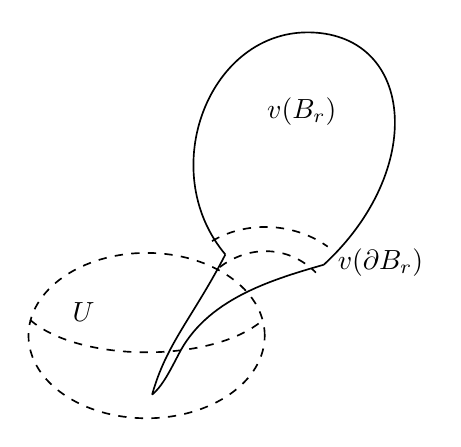
\begin{tikzpicture}[line width=0.6pt]
  \draw[dashed] (-1.35,-1.75) ellipse (1.5 and 1.05);
  \draw[dashed] (-2.83,-1.55) .. controls (-2.2,-2.1) and (-0.5,-2.1) .. (0.13,-1.55);
  \draw (-0.35,-0.72) .. controls (-0.75,-1.5) and (-1.1,-1.85) .. (-1.28,-2.5);
  \draw (0.9,-0.85) .. controls (0.2,-1.05) and (-0.6,-1.3) .. (-0.95,-2.0)
        .. controls (-1.08,-2.25) and (-1.16,-2.4) .. (-1.28,-2.5);
  \draw (-0.35,-0.72) .. controls (-1.25,0.35) and (-0.55,2.15) .. (0.75,2.1)
        .. controls (2.05,2.05) and (2.2,0.35) .. (0.9,-0.85);
  \draw[dashed] (-0.52,-0.55) .. controls (-0.1,-0.3) and (0.5,-0.3) .. (0.95,-0.62);
  \draw[dashed] (-0.42,-0.88) .. controls (-0.05,-0.6) and (0.45,-0.6) .. (0.8,-0.95);
  \node at (0.62,1.1) {$v(B_r)$};
  \node at (1.62,-0.82) {$v(\partial B_r)$};
  \node at (-2.15,-1.45) {$U$};
\end{tikzpicture}
\caption{一个\trBubble}
\label{fig:bubble-neck}
\end{figure}

至于第二个积分，它则\trConvergence{}于 $v(\RR^{2})$ 的面积，而该面积非零。这正是我们要找的矛盾。同心\trCircle{} $v(\partial B_r)$ 的周长越来越小，这正是这类对象被称作\trBubble{}的缘由；见\cref{fig:bubble-neck}。

\begin{proof}[\cref{thm:boundary-length-sequence}的证明]
由于 $v$ 是 $J$-\trHolomorphic{}的，\trForm{} $v^\star\omega$ 是 $\RR^2$ 上的一个\trSymplecticForm{}。因此它可以写成
\[
v^\star\omega_{(\rho,\theta)}=f(\rho,\theta)\,\rho\,d\theta\wedge d\rho
\]
其中 $f$ 是一个正函数。由于 $v$ 是 $J$-\trHolomorphic{}的，这个\trSymplecticForm{}连同通常的\trAlmostComplex{}结构一起给出了 $\RR^2$ 上的一个\trRiemann\trMetric，即 $f(\rho,\theta)(d\rho^2+\rho^2\,d\theta^2)$，利用它我们可以计算边界 $v(\partial B_r)$ 的长度 $\ell(r)$：
\[
\ell(r)=r\int_0^{2\pi}\sqrt{f(r,\theta)}\,d\theta\text{。}
\]
同样地，\footnote{译注：原书此段及上下两式共三处疑误，合并披露。其一，上文仅因 $v$ 是 $J$-\trHolomorphic{}的便称\trForm{} $v^\star\omega$ 是 $\RR^2$ 上的一个\trSymplecticForm{}、$f$ 是一个正函数；但 $J$-\trHolomorphic{}映射可以有分支点（例如 $v(z)=z^2$ 在 $z=0$ 处），故一般只能有 $v^\star\omega\ge 0$（即 $f\ge 0$，在分支点处为零）；好在随后的\trCauchy--\trSchwarz{}不等式与面积估计只需 $f\ge 0$，论证不受影响。其二，上一式楔积印作 $f(\rho,\theta)\,\rho\,d\theta\wedge d\rho$；按极坐标换算 $ds\wedge dt=\rho\,d\rho\wedge d\theta$，$d\theta$ 与 $d\rho$ 的先后次序疑应相反；照排存疑。其三，下一式迭次积分印作 $\int_0^{2\pi}\bigl(\int_0^r f(\rho,\theta)\,\rho\,d\theta\bigr)d\rho$，积分变量 $\theta$ 与 $\rho$ 内外倒置；据再下一行 $A'(r)=\int_0^{2\pi}f(r,\theta)\,r\,d\theta$ 反证，应为内层对 $\rho$ 积分、外层对 $\theta$ 积分；此处径改。——译者注}
\[
A(r)=\int_{B_r}v^\star\omega=\int_0^{2\pi}\Bigl(\int_0^r f(\rho,\theta)\,\rho\,d\rho\Bigr)d\theta\text{。}
\]
由此，
\[
A'(r)=\frac{dA}{dr}=\int_0^{2\pi}f(r,\theta)\,r\,d\theta\text{。}
\]
应用\trCauchy--\trSchwarz{}不等式，我们得到
\[
\ell(r)=r\int_0^{2\pi}\sqrt{f(r,\theta)}\,d\theta
\le r\sqrt{\int_0^{2\pi}\,d\theta\int_0^{2\pi}f(r,\theta)\,d\theta}
=r\sqrt{2\pi\,\frac{A'(r)}{r}}
\]
从而
\[
\ell(r)^2\le 2\pi rA'(r)\text{。}
\]
我们还需验证：由于函数 $r\mapsto A(r)$ 是\emph{\trBounded}的并且可微，故存在一列趋于 $+\infty$ 的 $r_k$，使得 $\lim r_kA'(r_k)=0$。这是一个容易的练习：由于 $A$ \trBounded，我们有
\[
\lim_{k\to+\infty}\frac{A(k^2)-A(k)}{\ln k}=0\text{。}
\]
这个商也可以写成
\[
\frac{A(k^2)-A(k)}{\ln k}=\frac{A(k^2)-A(k)}{\ln k^2-\ln k}=\frac{A'(r_k)}{(1/r_k)}
\]
其中由中值定理，$r_k$ 介于 $k$ 与 $k^2$ 之间（从而趋于无穷）。
\end{proof}

这就结束了\cref{thm:uniform-gradient-bound}的证明，从而也就结束了\trCompact{}性定理的证明。
\end{proof}

\subsection{$\CP^2(\CC)$ 中的一个\trBubble{}例子}

我们刚刚证明了：由于辛\trManifold{} $W$ 不含有任何具有非零辛面积的\trSphere，所以不可能有\trBubble。另一方面，如果确有 $\omega|_{\pi_2(W)}\neq 0$，那么一个涉及“可去\trSingularPoint”的论证使我们能把 $v$ 扩张到 $\CC\cup\{\infty\}$ 上，由此便得到我们称之为“\trBubble”的东西。

为了把情形弄清楚，让我们在复\trProjectivePlane{}中给出一个经典的\trBubble{}例子。注意，在这个辛\trManifold{}中是存在\trSphere{}的：一条\trProjective{}直线就是一个 $\CP^1(\CC)$，因而也是一个\trSphere{} $S^2$。此外，我们在\cref{sec:examples-symplectic-manifolds}中构造的\trSymplecticForm{}给予一切\trProjective{}直线以正的面积：一条\trProjective{}直线是一条复的（\trHolomorphic{}的）曲线，特别地，限制在这类曲线上的\trSymplecticForm{}是一个\trVolume{}形式。因此，复\trProjective{}空间不满足我们的条件。我们在这里给出的例子是可能的最简单的例子：我们观察一族\trDegenerate{}成两条直线之并集的\trSmooth{}\trConic。

\begin{figure}[htbp]
\centering
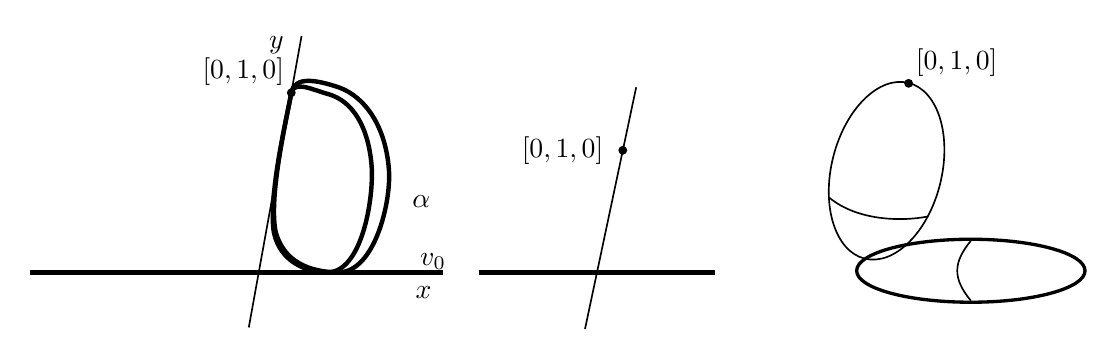
\begin{tikzpicture}[line width=0.6pt]
  \draw[line width=1.6pt] (-2.5,0) -- (2.75,0);
  \node[below=1pt] at (2.5,-0.02) {$x$};
  \node at (2.62,0.14) {$v_0$};
  \draw (0.28,-0.7) -- (0.95,3.0);
  \node[left=2pt] at (0.92,2.88) {$y$};
  \draw[line width=1.6pt] (0.82,2.28)
        .. controls (0.86,2.5) and (1.15,2.44) .. (1.42,2.35)
        .. controls (1.76,2.23) and (2.02,1.85) .. (2.06,1.3)
        .. controls (2.09,0.9) and (1.88,0.0) .. (1.42,0.0)
        .. controls (1.06,0.0) and (0.72,0.13) .. (0.62,0.52)
        .. controls (0.53,0.98) and (0.77,1.99) .. (0.82,2.28) -- cycle;
  \node[right=2pt] at (2.16,0.9) {$\alpha$};
  \draw[line width=1.6pt] (0.82,2.28)
        .. controls (0.86,2.44) and (1.08,2.32) .. (1.3,2.26)
        .. controls (1.6,2.17) and (1.8,1.85) .. (1.84,1.35)
        .. controls (1.87,0.95) and (1.72,0.0) .. (1.28,0.0)
        .. controls (1.0,0.0) and (0.68,0.14) .. (0.6,0.5)
        .. controls (0.52,0.95) and (0.76,1.95) .. (0.82,2.28) -- cycle;
  \fill (0.82,2.28) circle (1.6pt);
  \node[above left=-1pt] at (0.82,2.28) {$[0,1,0]$};
  \begin{scope}[shift={(4.7,0)}]
    \draw[line width=1.6pt] (-1.5,0) -- (1.5,0);
    \draw (-0.15,-0.72) -- (0.5,2.35);
    \fill (0.33,1.55) circle (1.6pt);
    \node[left=2pt] at (0.28,1.55) {$[0,1,0]$};
  \end{scope}
  \begin{scope}[shift={(8.2,0)}]
    \draw[line width=1.2pt] (1.25,0.02) ellipse (1.45 and 0.4);
    \draw (1.25,-0.36) .. controls (1.02,-0.08) and (1.02,0.12) .. (1.25,0.4);
    \draw[rotate around={-14:(0.18,1.29)}] (0.18,1.29) ellipse (0.7 and 1.15);
    \draw (-0.55,0.95) .. controls (-0.2,0.66) and (0.35,0.64) .. (0.71,0.71);
    \fill (0.46,2.4) circle (1.6pt);
    \node[above right=-1pt] at (0.46,2.4) {$[0,1,0]$};
  \end{scope}
\end{tikzpicture}
\caption{}
\label{fig:conic-bubble}
\end{figure}

对每个 $\alpha\in\CC$，我们考虑曲线（\trConic）
\[
\begin{aligned}
v_\alpha\colon\CP^1(\CC)&\longrightarrow\CP^2(\CC)\\
{[x,y]}&\longmapsto[x^2,\alpha y^2,xy]\text{，}
\end{aligned}
\]
这不过是
\[
\begin{aligned}
v_\alpha\colon\CC&\longrightarrow\CC^2\\
z&\longmapsto(z,\alpha/z)
\end{aligned}
\]
的\trCompactification{}而已。

当 $\alpha=0$ 时，像是“$x$ 轴”。当 $\alpha\neq 0$ 时，它是一条\trConic。$v_\alpha$ 的所有像曲线都包含 $y$ 轴上的无穷远点，即在\trHomogeneousCoordinates{}下为 $[0,1,0]$ 的那个点。\footnote{译注：原书此例有三处从简，照排于此，归组备案。其一，齐次式 $[x^{2},\alpha y^{2},xy]$ 在 $\alpha=0$ 且 $[x,y]=[0,1]$ 时给出 $[0,0,0]$，并无定义（下文“极限曲线并\emph{不}是一个映射 $v_{0}$ 的像”一句即指此）；其二，仿射式 $z\mapsto(z,\alpha/z)$ 的定义域应是 $\CC^{\star}$（$z=0$ 处 $\alpha/z$ 无意义；$\alpha=0$ 时虽可延拓到 $z=0$，式子本身如此）；其三，“所有像曲线都包含 $[0,1,0]$”仅当 $\alpha\neq0$ 时成立（$\alpha=0$ 的像是 $x$ 轴的\trProjective{}闭包，不含 $y$ 轴上的无穷远点）。——译者注}当 $\alpha$ 趋于 $0$ 时，这个点便“给自己吹出了一个\trBubble”。\cref{fig:conic-bubble}通过展示\trConic{} $v_\alpha(\CP^1(\CC))$ 与极限“曲线”（也就是 $x$ 轴与 $y$ 轴）的各种状态来阐明这一情形，它们被表现为：
\begin{itemize}
\item 一朝是两条相交的直线；
\item 另一朝是一条“带\trBubble{}的曲线”，在这幅图中，两条复\trProjective{}直线各自被表示成一个\trSphere{} $S^2$。
\end{itemize}
我们还注意到：
\begin{itemize}
\item 极限曲线并\emph{不}是一个映射 $v_0\colon\CP^1(\CC)\to\CP^2(\CC)$ 的像。
\item 然而，它在去掉点 $0=[0,1]$ 之后的补集上确实有一个极限，即 $z\mapsto(z,0)$。
\item \trCircle{} $|z|^2=\alpha$ 是一个\trDisk{}（$|z|^2\le\alpha$）的边界，而这个\trDisk{}在像中所占的地方越来越大；见\cref{fig:disk-boundary}。
\end{itemize}

\begin{figure}[htbp]
\centering
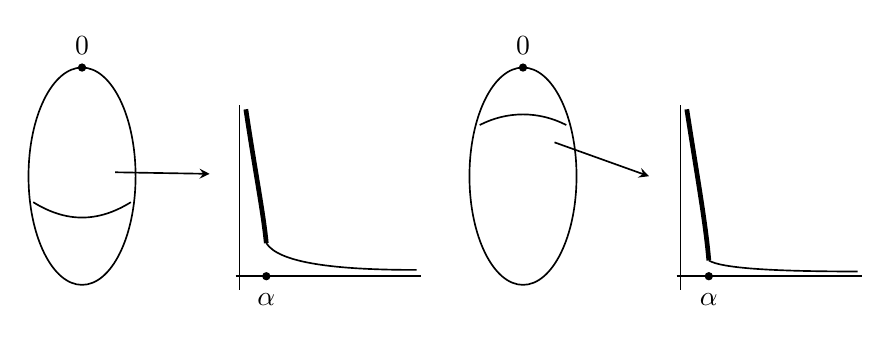
\begin{tikzpicture}[line width=0.6pt,>=stealth]
  \begin{scope}
    \draw (0,0.95) ellipse (0.68 and 1.38);
    \fill (0,2.33) circle (1.5pt);
    \node[above=1pt] at (0,2.33) {$0$};
    \draw (-0.62,0.62) .. controls (-0.2,0.36) and (0.2,0.36) .. (0.62,0.62);
    \draw[->] (0.42,1.0) -- (1.62,0.98);
    \draw (2.0,1.85) -- (2.0,-0.5);
    \draw (1.95,-0.32) -- (4.3,-0.32);
    \draw[line width=1.7pt] (2.08,1.8) .. controls (2.2,1.0) and (2.3,0.5) .. (2.34,0.1);
    \draw (2.34,0.1) .. controls (2.5,-0.15) and (3.2,-0.24) .. (4.25,-0.24);
    \fill (2.34,-0.32) circle (1.5pt);
    \node[below=2pt] at (2.34,-0.34) {$\alpha$};
  \end{scope}
  \begin{scope}[shift={(5.6,0)}]
    \draw (0,0.95) ellipse (0.68 and 1.38);
    \fill (0,2.33) circle (1.5pt);
    \node[above=1pt] at (0,2.33) {$0$};
    \draw (-0.55,1.6) .. controls (-0.2,1.78) and (0.2,1.78) .. (0.55,1.6);
    \draw[->] (0.4,1.38) -- (1.6,0.95);
    \draw (2.0,1.85) -- (2.0,-0.5);
    \draw (1.95,-0.32) -- (4.3,-0.32);
    \draw[line width=1.7pt] (2.08,1.8) .. controls (2.22,0.9) and (2.32,0.35) .. (2.36,-0.12);
    \draw (2.36,-0.12) .. controls (2.52,-0.22) and (3.2,-0.26) .. (4.25,-0.26);
    \fill (2.36,-0.32) circle (1.5pt);
    \node[below=2pt] at (2.36,-0.34) {$\alpha$};
  \end{scope}
\end{tikzpicture}
\caption{}
\label{fig:disk-boundary}
\end{figure}
